\documentclass[11pt,a4paper]{article}
\usepackage[margin=2.2cm]{geometry}
\usepackage{graphicx}
\usepackage{booktabs}
\usepackage{xcolor}
\usepackage{tcolorbox}
\usepackage{hyperref}
\usepackage{caption}
\usepackage{float}
\usepackage{fancyhdr}
\usepackage{titlesec}
\usepackage{enumitem}
\usepackage{tabularx}
\definecolor{navy}{HTML}{1F3A5F}
\definecolor{teal}{HTML}{2A9D8F}
\definecolor{red}{HTML}{C8553D}
\definecolor{grey}{HTML}{8D99AE}
\hypersetup{colorlinks=true,linkcolor=navy,urlcolor=teal}
\titleformat{\section}{\Large\bfseries\color{navy}}{\thesection}{0.6em}{}
\titleformat{\subsection}{\large\bfseries\color{navy}}{\thesubsection}{0.5em}{}
\pagestyle{fancy}\fancyhf{}
\fancyhead[L]{\small\color{grey}Zinger market making: results, capital and economics}
\fancyhead[R]{\small\color{grey}21 October 2026}
\fancyfoot[C]{\small\thepage}
\setlength{\parskip}{0.5em}
\newtcolorbox{callout}[1][]{colback=teal!8,colframe=teal,boxrule=0.6pt,arc=2pt,left=8pt,right=8pt,top=6pt,bottom=6pt,#1}
\newtcolorbox{warn}{colback=red!7,colframe=red,boxrule=0.6pt,arc=2pt,left=8pt,right=8pt,top=6pt,bottom=6pt}
\captionsetup{font=small,labelfont=bf,labelformat=simple,labelsep=period}
\graphicspath{{../figures/}}
\newcolumntype{Y}{>{\raggedright\arraybackslash}X}

\title{\textcolor{navy}{\textbf{Zinger Market Making on Polymarket}}\\[0.3em]
\large Results to date, capital simulation and per-\$100 economics}
\author{Research record \\ Paper trading and public market data only}
\date{21 October 2026 (UTC) \quad Supersedes the 19-hour interim edition}

\begin{document}
\maketitle
\thispagestyle{empty}

\begin{callout}
\textbf{Status and risk disclosure.}\\
No order has been placed and no money spent. Every figure is a simulation on live public data.
On the full 24-hour recording, quote settings chosen on the first half \textbf{lost \$42.44 per day on about \$13,000 (\,$-$0.33\% per day) on the unseen second half}. The 19-hour interim showed +0.14\% per day; that gain did not hold.
Most markets made a little; three large adverse moves outweighed them. Real capital remains conditional on the gates in Section~\ref{sec:gates}.
\end{callout}

\section{Summary}
\begin{itemize}[leftmargin=1.2em]
  \item \textbf{Reward capture works mechanically.} After fixing churn and stale-book handling, the runner earns a projected reward share in every market it quotes. Liquid markets paid a steady \$10--14 per day at minimum size across 40 markets.
  \item \textbf{Fill losses decide the result.} Over the full day, adverse fills cost more than the reward at every quote distance when one setting is used for all markets.
  \item \textbf{Split-sample test, full day.} Per-market settings chosen on the first half returned $-$0.33\% per day on the second half for liquid markets and $-$2.77\% for thin books. Capping size at the reward minimum gave the same rate; losses scale with size.
  \item \textbf{Losses are concentrated.} Three liquid markets lost \$71.44 per day between them; the other 37 made +\$29.00. The median market made +\$0.53 per day.
  \item \textbf{Capital simulation.} Small books (\$100--\$1,000, 2--9 markets) were positive on the second half; books of \$2,500 and above lost about 0.3\% per day.
  \item \textbf{Expectation.} No positive edge is demonstrated. The profile is small steady gains with occasional large losses, which needs news and jump protection before any further sizing.
\end{itemize}

\section{What was built}
\begin{table}[H]\centering\small
\begin{tabularx}{\linewidth}{@{}p{4.3cm}Y@{}}
\toprule
Component & Purpose \\
\midrule
Paper market-making runner & Quotes against live books; simulates queue position, fills, inventory, fees and recovery; zero orders \\
Resting quotes & Orders keep their queue position while the target stays within one tick \\
Connection-health freshness & A book counts as current while its websocket answers a one-second heartbeat \\
Reward accrual & Polymarket's quadratic reward score, sampled each minute, kept separate from cash \\
Market scanner & Every reward-eligible market from the CLOB, ranked by projected reward per \$100 \\
Recorder & One snapshot per minute of every book level inside the reward band, plus trades \\
Optimiser and split test & Sweeps quote distance and size per market with a pessimistic fill cost; tests settings on unseen data \\
Capital simulator & Allocates a budget across markets in first-half rank order and scores it on the second half \\
\bottomrule
\end{tabularx}
\caption{Components built during the research.}
\end{table}

\section{Execution results from the paper runner}
\begin{figure}[H]\centering
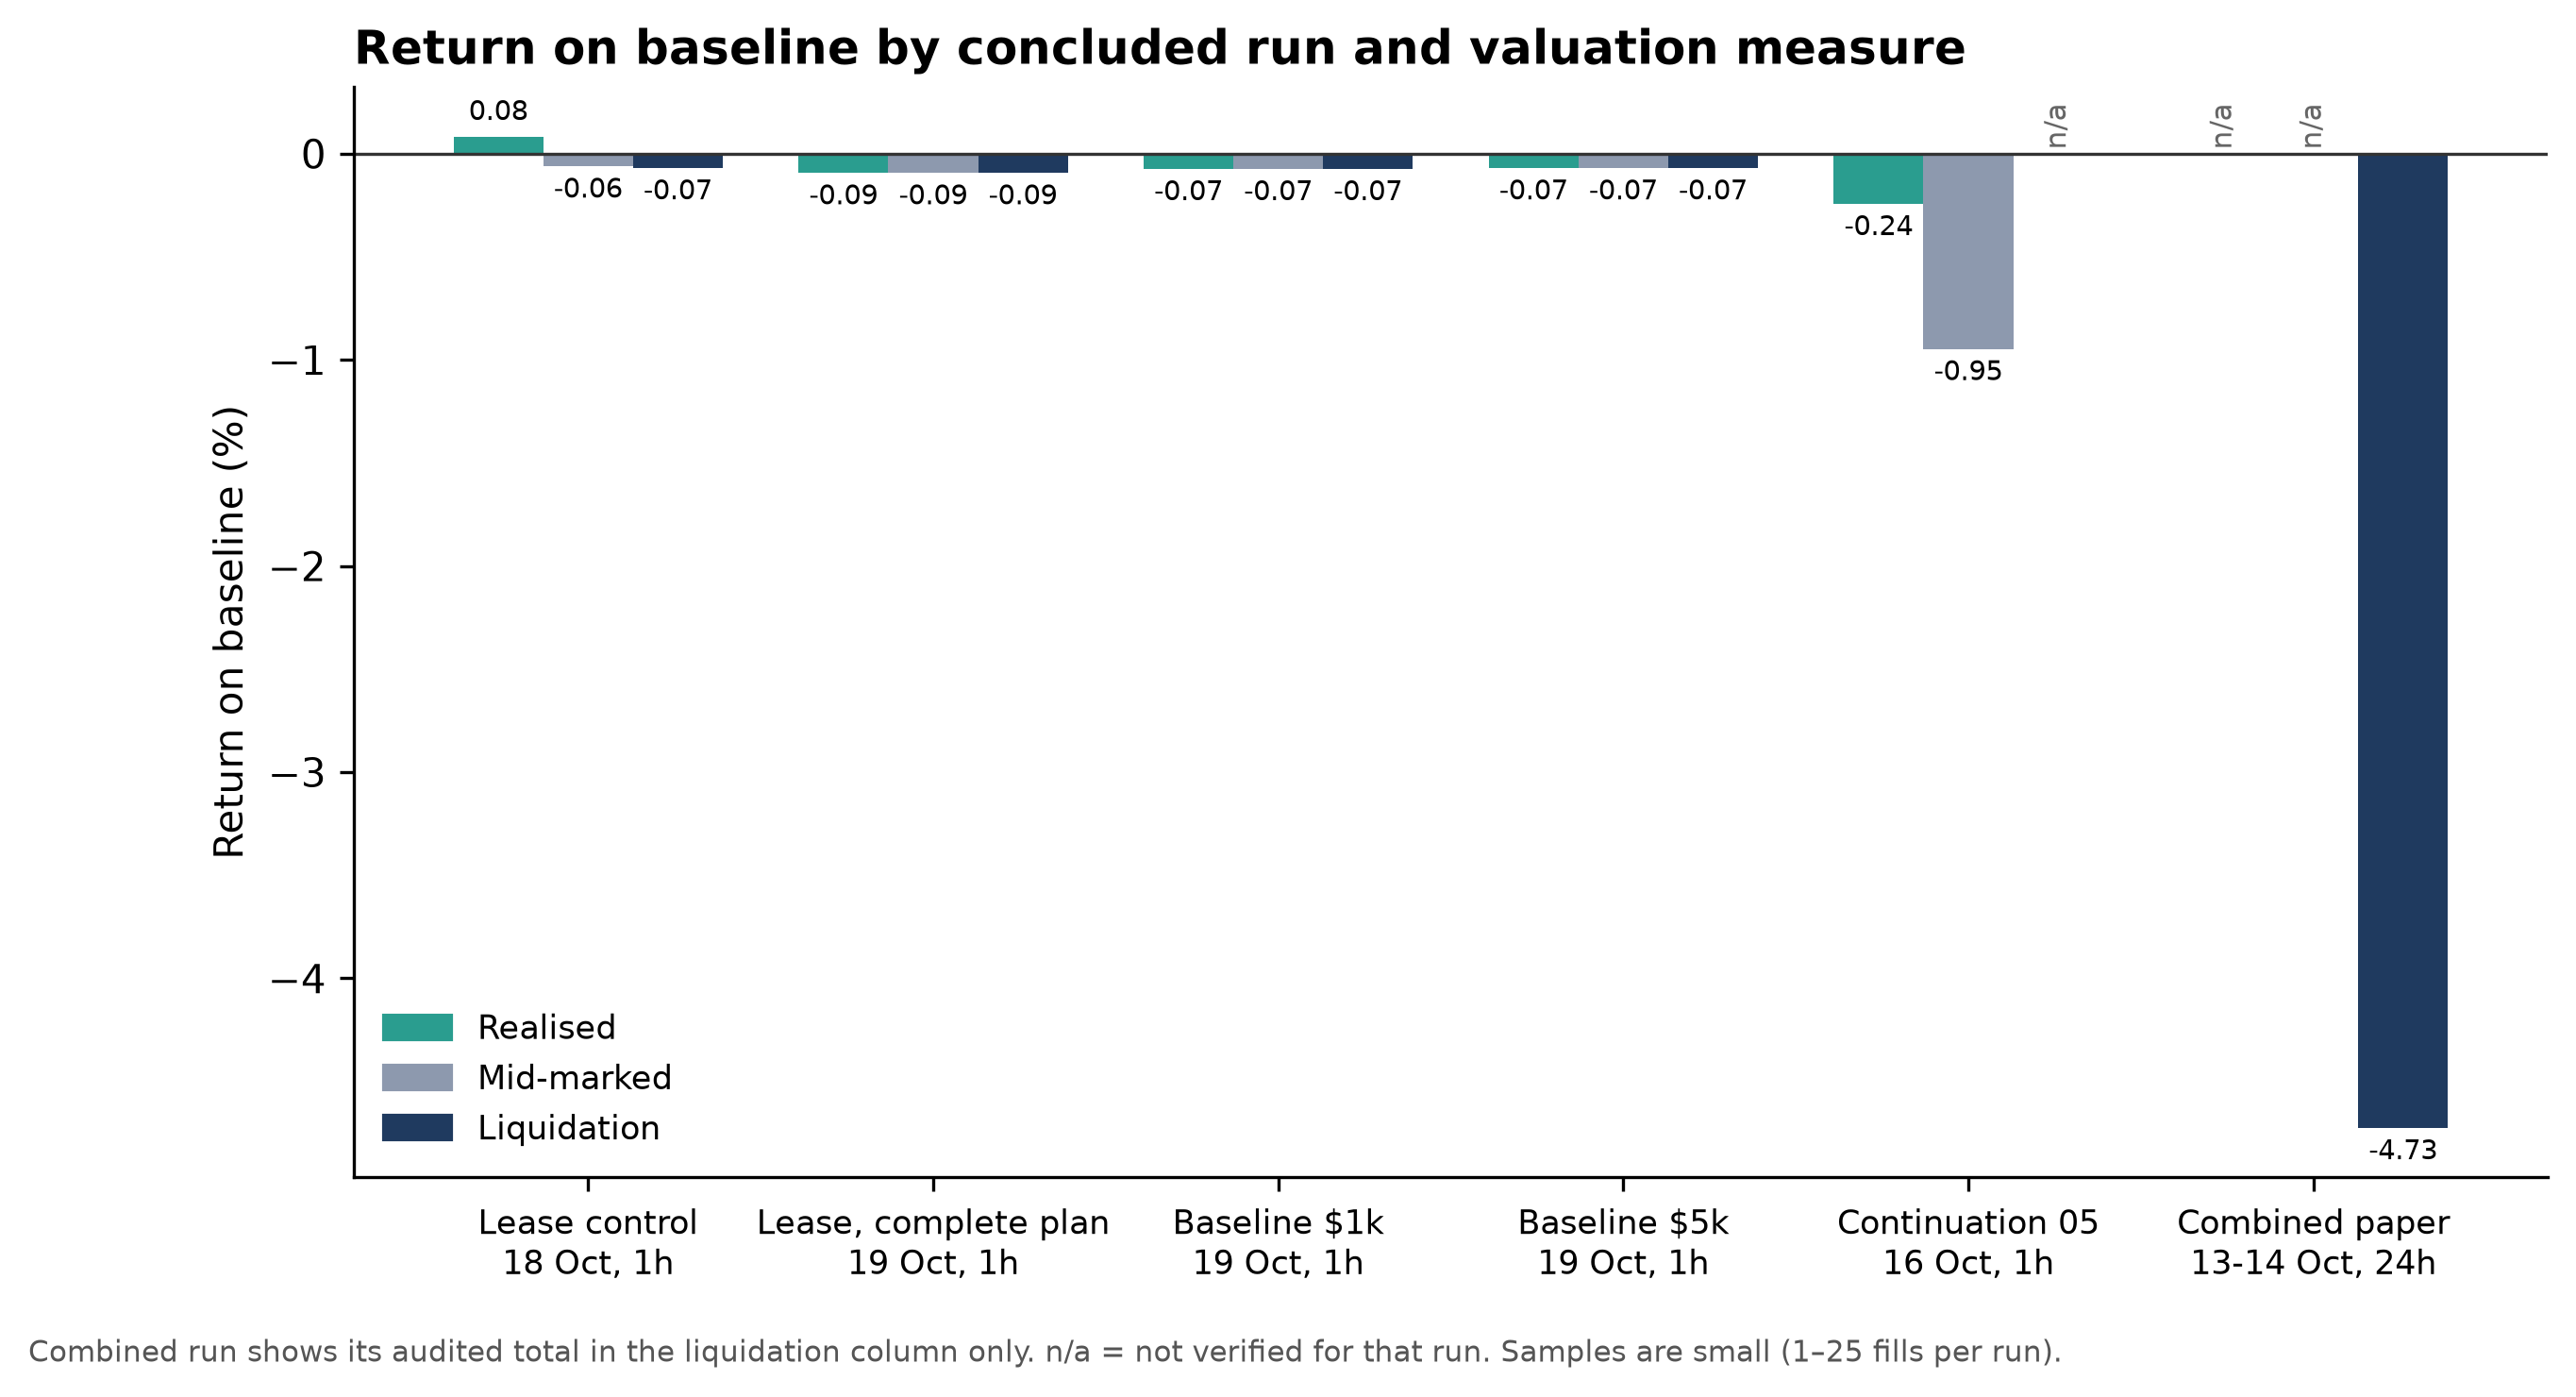
\includegraphics[width=\linewidth]{runs-return-pct}
\caption{Return on baseline for each concluded paper run (1--25 fills per run).}
\end{figure}

\begin{table}[H]\centering\small
\begin{tabular}{@{}lrrrr@{}}
\toprule
Run & Baseline & Fills & Liquidation P/L & Return \\
\midrule
Lease control, 18 Oct, 1 h & \$1,000 & 1 & $-$\$0.70 & $-$0.07\% \\
Lease, complete plan, 19 Oct, 1 h & \$1,000 & 2 & $-$\$0.94 & $-$0.09\% \\
Baseline \$1k, 19 Oct, 1 h & \$1,000 & 2 & $-$\$0.74 & $-$0.07\% \\
Baseline \$5k, 19 Oct, 1 h & \$5,000 & 2 & $-$\$3.51 & $-$0.07\% \\
Continuation 05, 16 Oct, 1 h & \$1,000 & 25 & not verified & realised $-$0.24\% \\
Combined paper, 13--14 Oct, 24 h & \$2,000 & --- & $-$\$94.52 & $-$4.73\% \\
\bottomrule
\end{tabular}
\caption{Concluded paper runs. Total simulated MM volume was about \$92.}
\end{table}

\section{What broke, and what was fixed}
\begin{table}[H]\centering\small
\begin{tabularx}{\linewidth}{@{}p{3.6cm}YY@{}}
\toprule
Problem & Effect & Fix \\
\midrule
Startup wait with no deadline & Three captures ran 17 hours with no data & Startup deadline, data watchdog, hard stop, one capture at a time \\
1.5\,s REST freshness rule & Books stale 72\% of the time & Websocket heartbeat freshness; stale share 0.7\% \\
Quotes expiring every 10\,s & Constant loss of queue position & Resting quotes with a one-tick tolerance \\
Trade endpoint ignores its window & Wrong volume, missed fills & Cursor paging filtered to each sample window \\
Snapshots kept the far end of the book & Early recordings unusable for re-scoring & Levels selected by distance from the midpoint \\
Single-snapshot reward estimates & \$8,752/day on thin books & Competition floor, then a 24-hour recording \\
Minute-cadence stub quotes & +\$70/day mostly from one news shock and one live game & Stub used only for reward share \\
\bottomrule
\end{tabularx}
\caption{Defects found and corrected.}
\end{table}

\section{Benchmark against an open-source market maker}
\begin{figure}[H]\centering
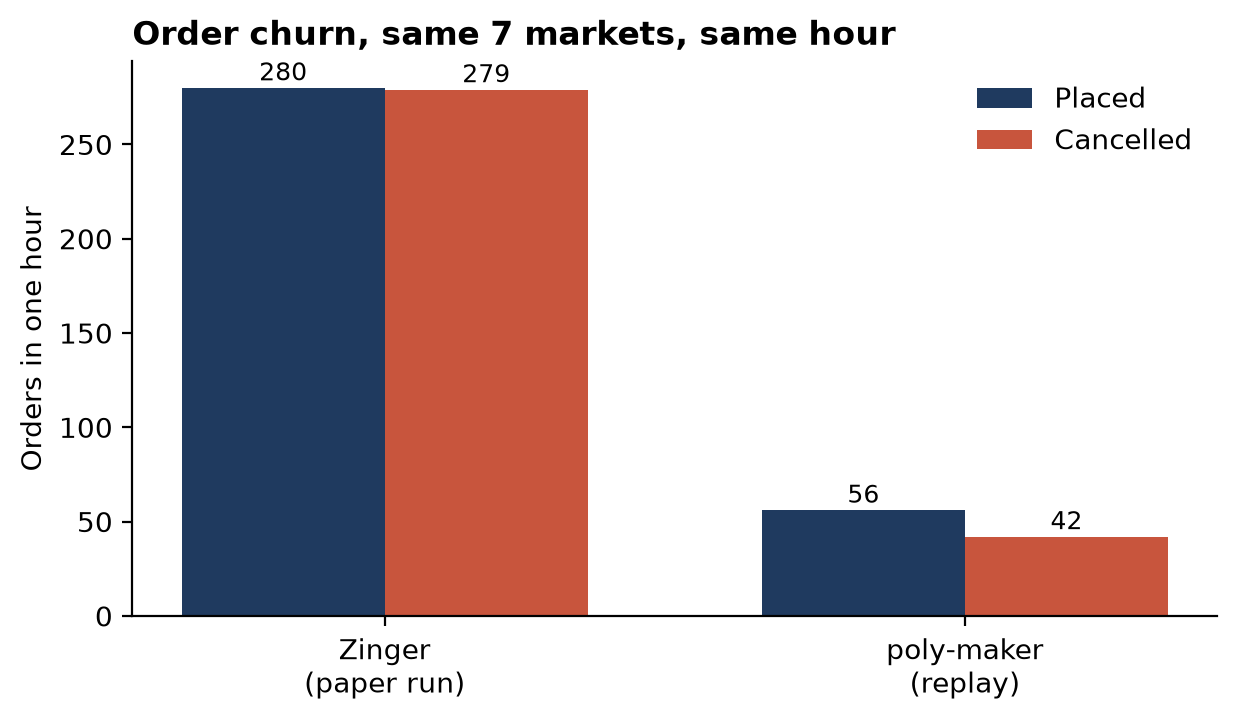
\includegraphics[width=0.48\linewidth]{bench1_churn}\hfill
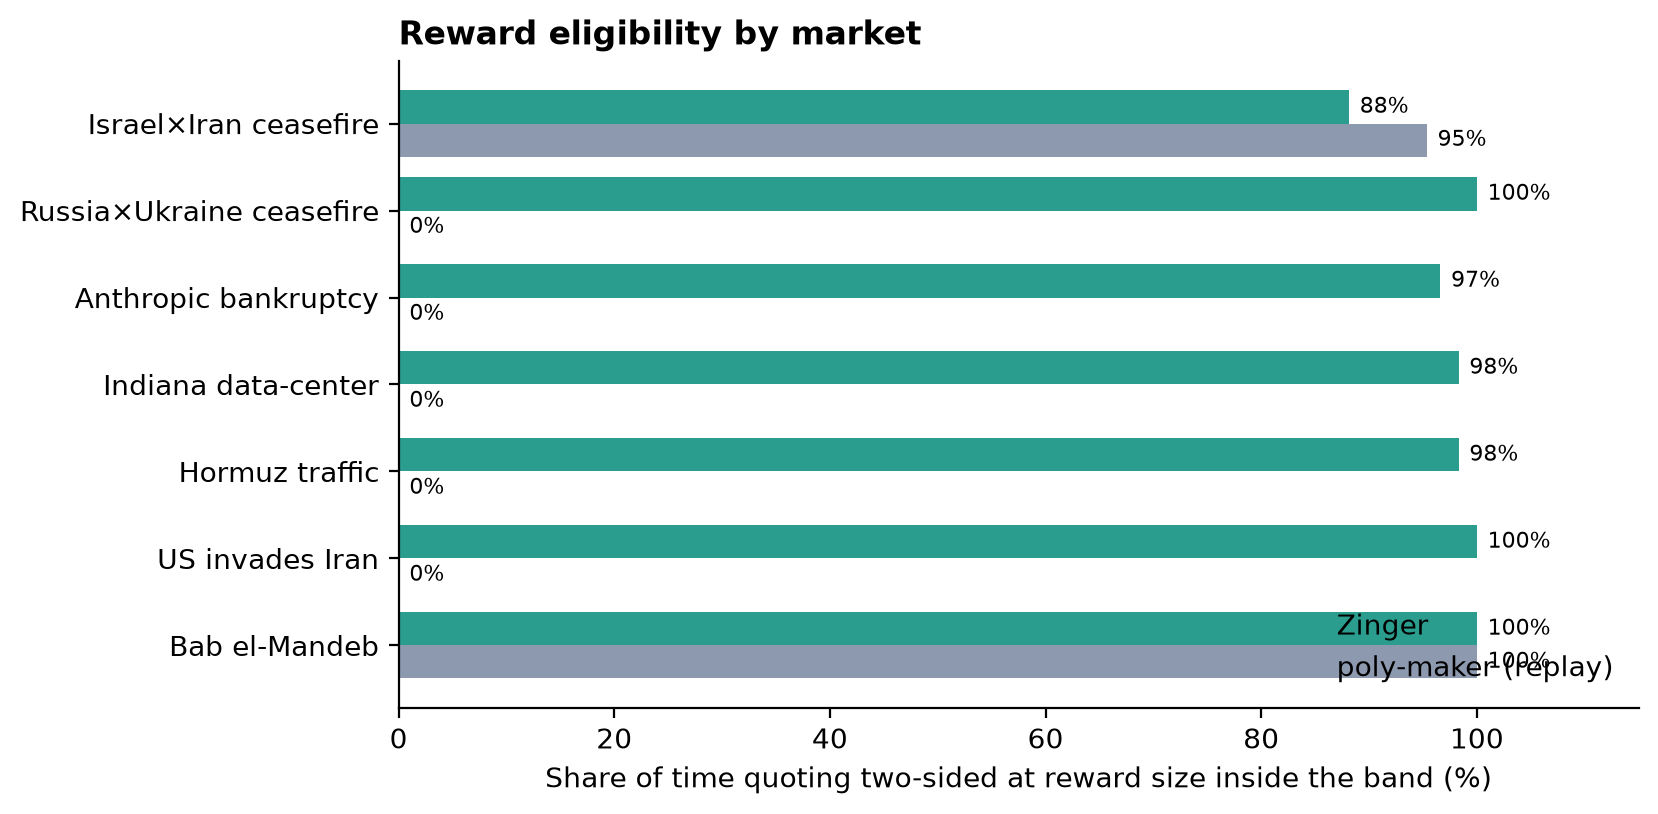
\includegraphics[width=0.5\linewidth]{bench2_eligibility}
\caption{Same 7 markets, same hour. Left: orders placed and cancelled. Right: time quoting two-sided at reward size inside the band.}
\end{figure}
Zinger churned five times more than \texttt{poly-maker}'s logic but qualified for rewards in all 7 markets; \texttt{poly-maker}'s copied profile under-sized its NO bids in 5. \texttt{poly-maker}'s own notes report a live loss of \$15.51 from one oversized fill, the same failure mode seen here.

\section{Market reach}
\begin{figure}[H]\centering
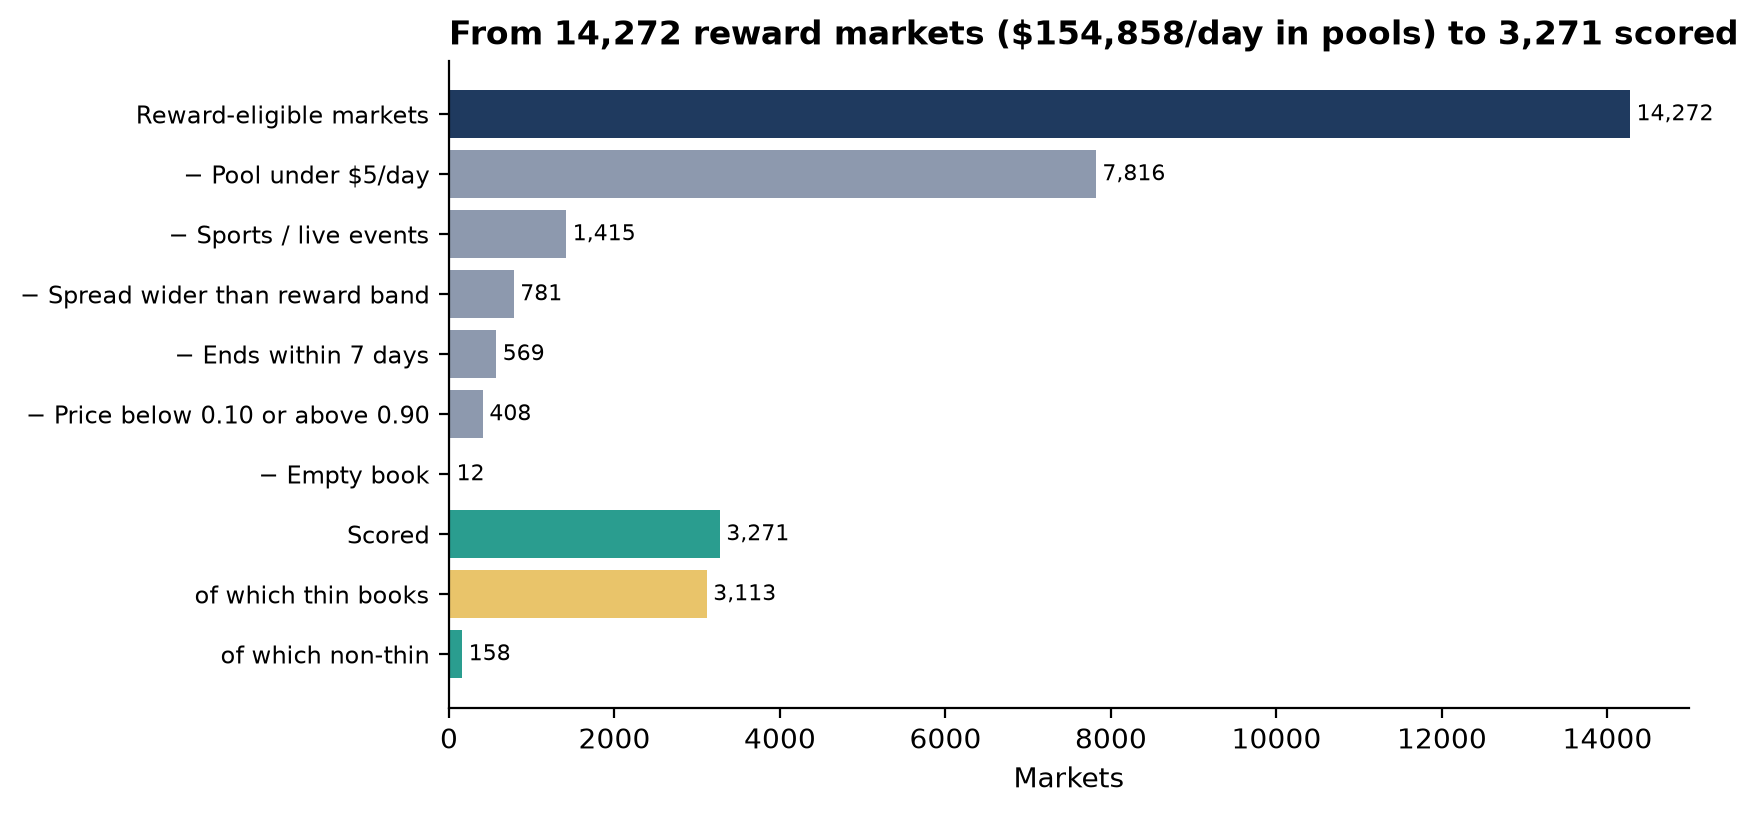
\includegraphics[width=0.88\linewidth]{scan-funnel}
\caption{14,272 reward markets (\$154,858 per day in pools) narrowed to 3,271 scored: 158 liquid, 3,113 thin.}
\end{figure}
\begin{figure}[H]\centering
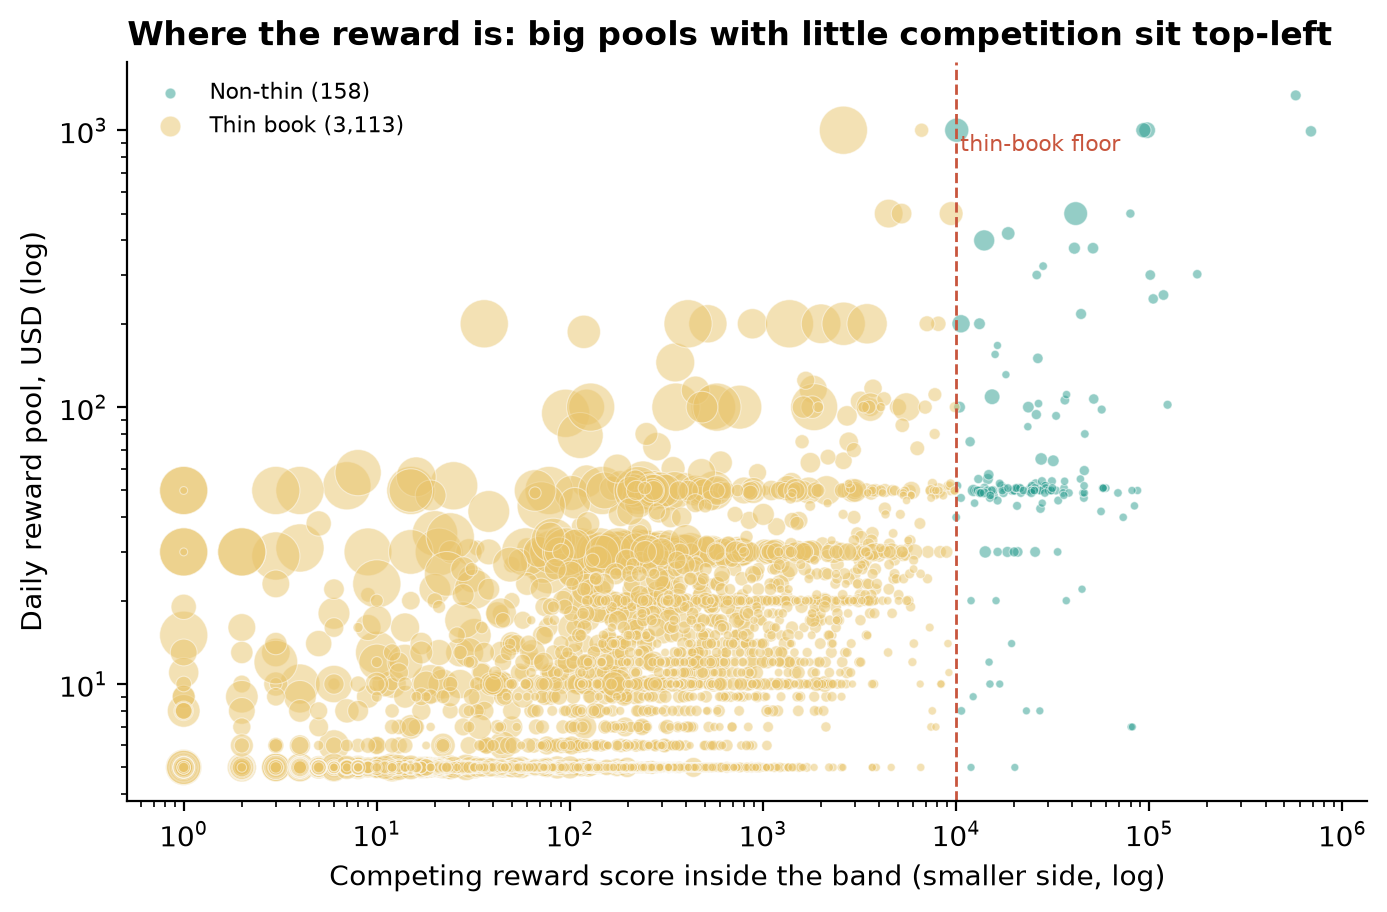
\includegraphics[width=0.82\linewidth]{scan-pool-vs-competition}
\caption{Daily pool against competing reward score.}
\end{figure}

\section{24-hour recording}
80 markets (40 liquid, 40 thin) were recorded once a minute from 20 October 18:40 UTC to 21 October 18:40 UTC: 1,440 minutes, 105,449 samples, no errors.
\begin{figure}[H]\centering
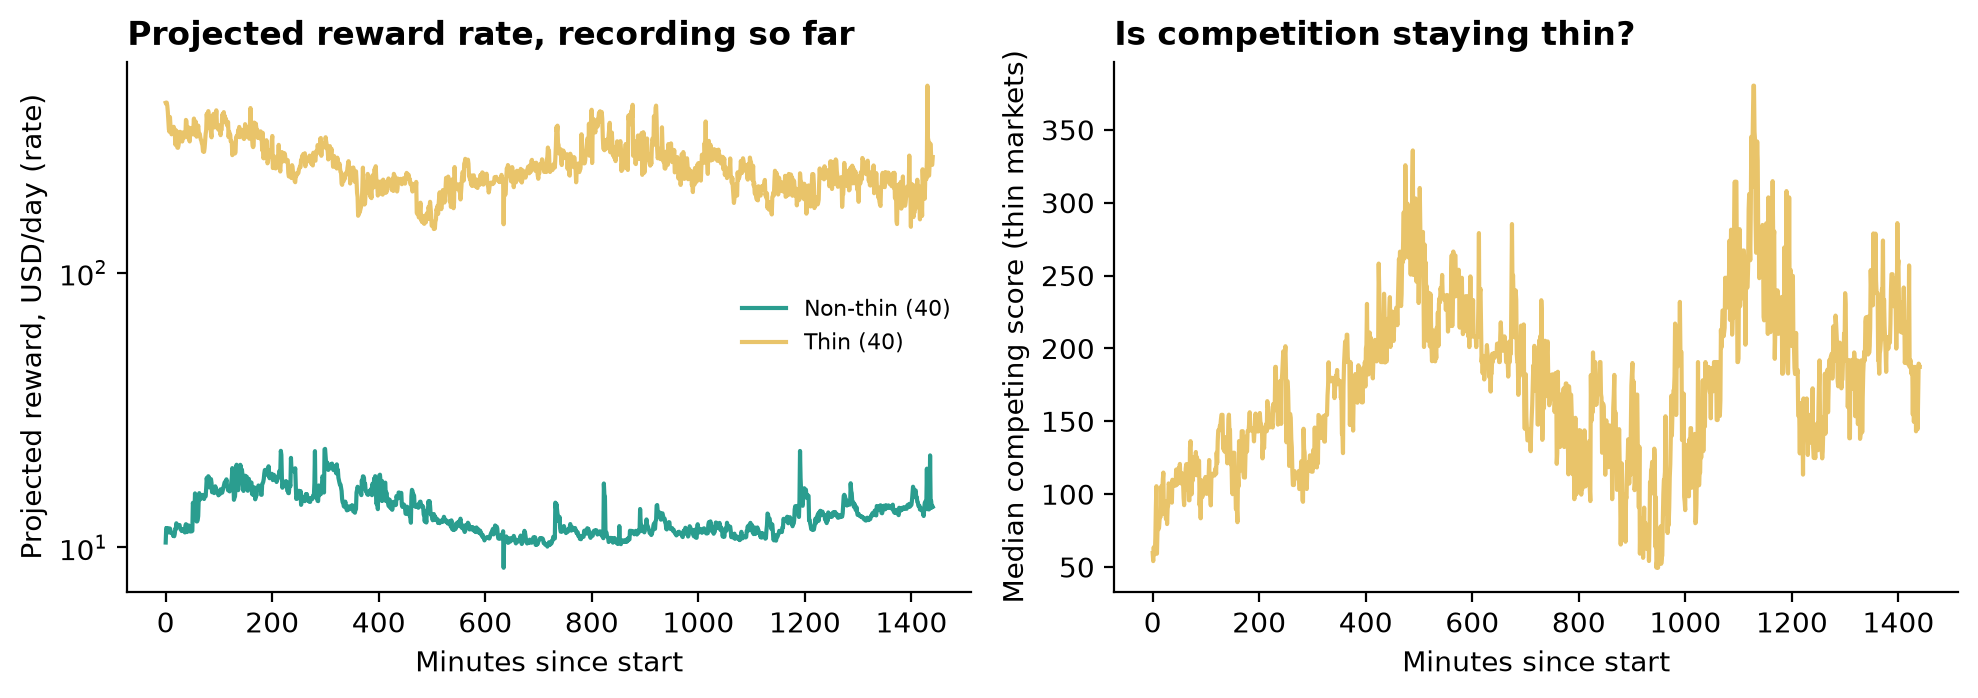
\includegraphics[width=\linewidth]{scan-recording}
\caption{Left: projected reward rate by group. Right: median competing score on thin markets.}
\end{figure}
\begin{table}[H]\centering\small
\begin{tabular}{@{}lrrr@{}}
\toprule
 & First minute & Last minute & Average \\
\midrule
Liquid projected reward & \$10.4/day & \$14.1/day & \$13.4/day \\
Thin projected reward & \$414/day & \$263/day & \$246/day \\
Thin median competing score & 60 & 187 & --- \\
\bottomrule
\end{tabular}
\caption{Reward before fill costs. Liquid rewards were stable; thin rewards fell as competition arrived.}
\end{table}

\section{Parameter tests}\label{sec:opt}
For each market-minute the optimiser tries 0--3 ticks back from the touch at 1, 2 and 4 times the reward minimum. Reward is scored against the recorded book. Fill cost is pessimistic: a fill counts only when the price moves through the quote and is marked 10 minutes later; benign fills that would earn spread are ignored.

\begin{figure}[H]\centering
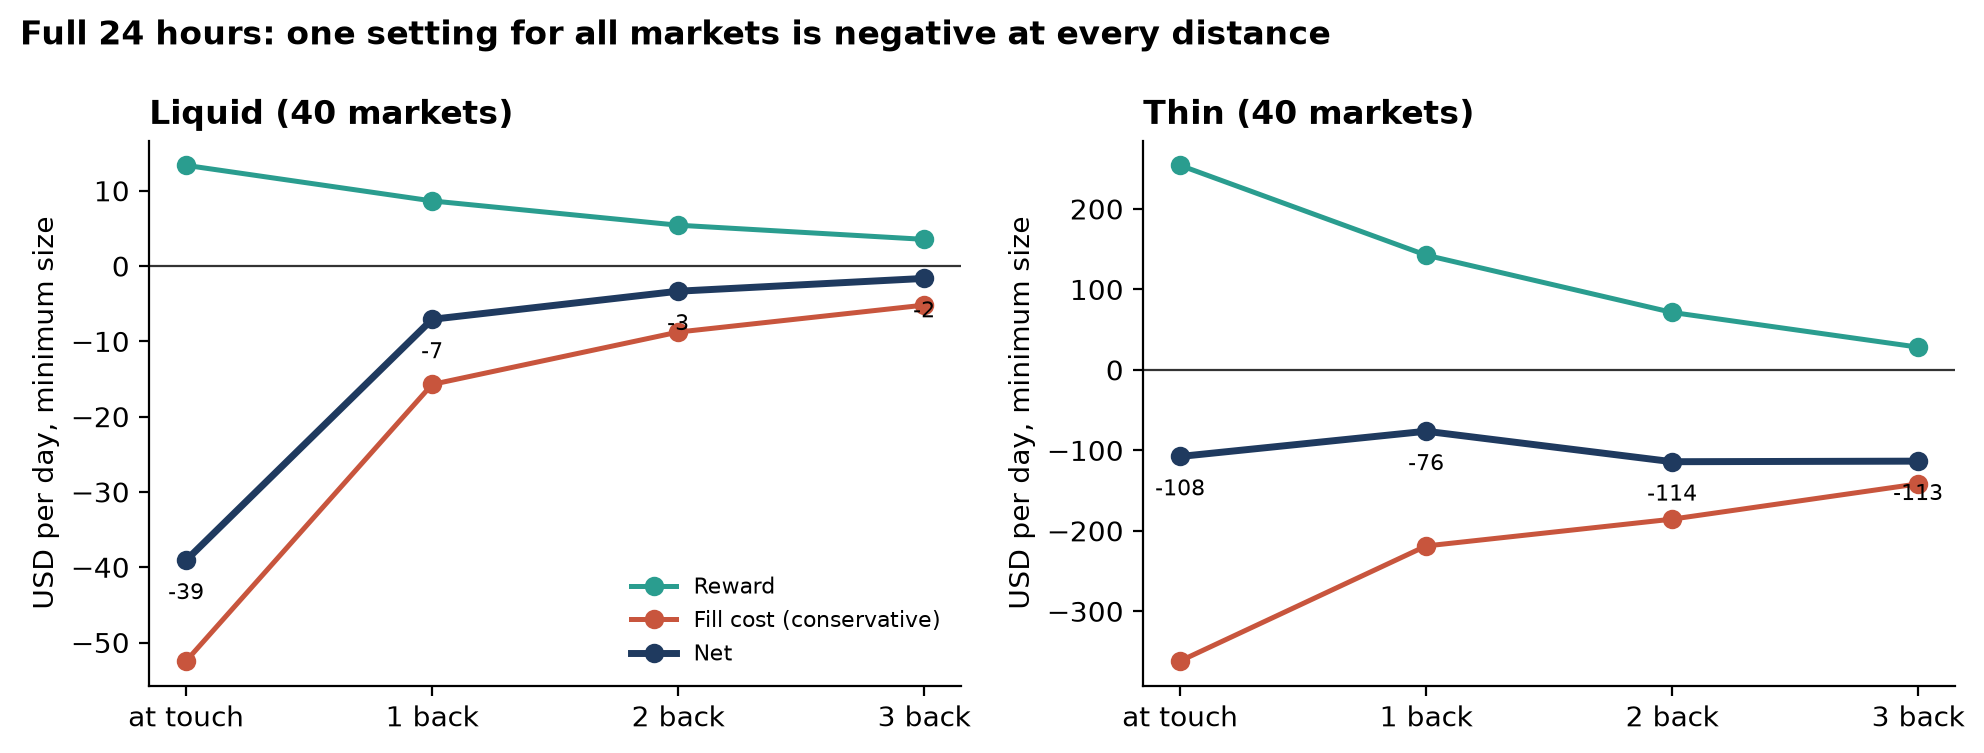
\includegraphics[width=\linewidth]{offset-curves-final}
\caption{Reward, fill cost and net by quote distance at minimum size, full 24 hours.}
\end{figure}
\begin{table}[H]\centering\small
\begin{tabular}{@{}lrrrrr@{}}
\toprule
Liquid, one setting & Reward & Fill cost & Net & Net \%/day & Fills/day \\
\midrule
At the touch & \$13.37 & $-$\$52.45 & $-$\$39.08 & $-$1.13\% & 354 \\
1 tick back & \$8.65 & $-$\$15.72 & $-$\$7.07 & $-$0.21\% & 36 \\
2 ticks back & \$5.43 & $-$\$8.77 & $-$\$3.34 & $-$0.10\% & 20 \\
3 ticks back & \$3.55 & $-$\$5.19 & $-$\$1.64 & $-$0.05\% & 9 \\
\bottomrule
\end{tabular}
\caption{Thin markets were negative at every distance ($-$\$76 to $-$\$114 per day).}
\end{table}

\subsection{More interactions lower returns}
\begin{figure}[H]\centering
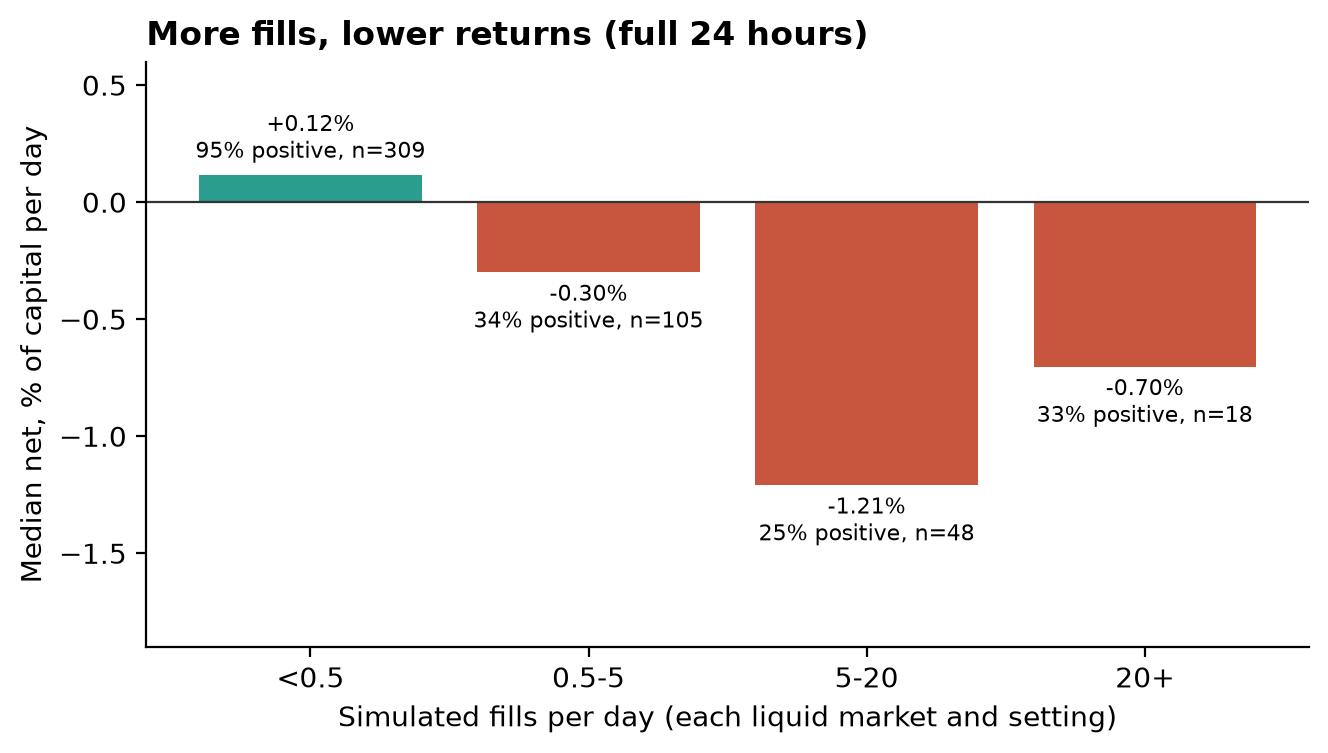
\includegraphics[width=0.78\linewidth]{interaction-final}
\caption{Every liquid market and setting, grouped by simulated fills per day.}
\end{figure}
Settings with almost no fills earned a median +0.12\% per day (95\% positive); 5--20 fills per day earned a median $-$1.21\%. Quoting faster or closer increases fills and lowers returns.

\subsection{Split-sample test}
\begin{figure}[H]\centering
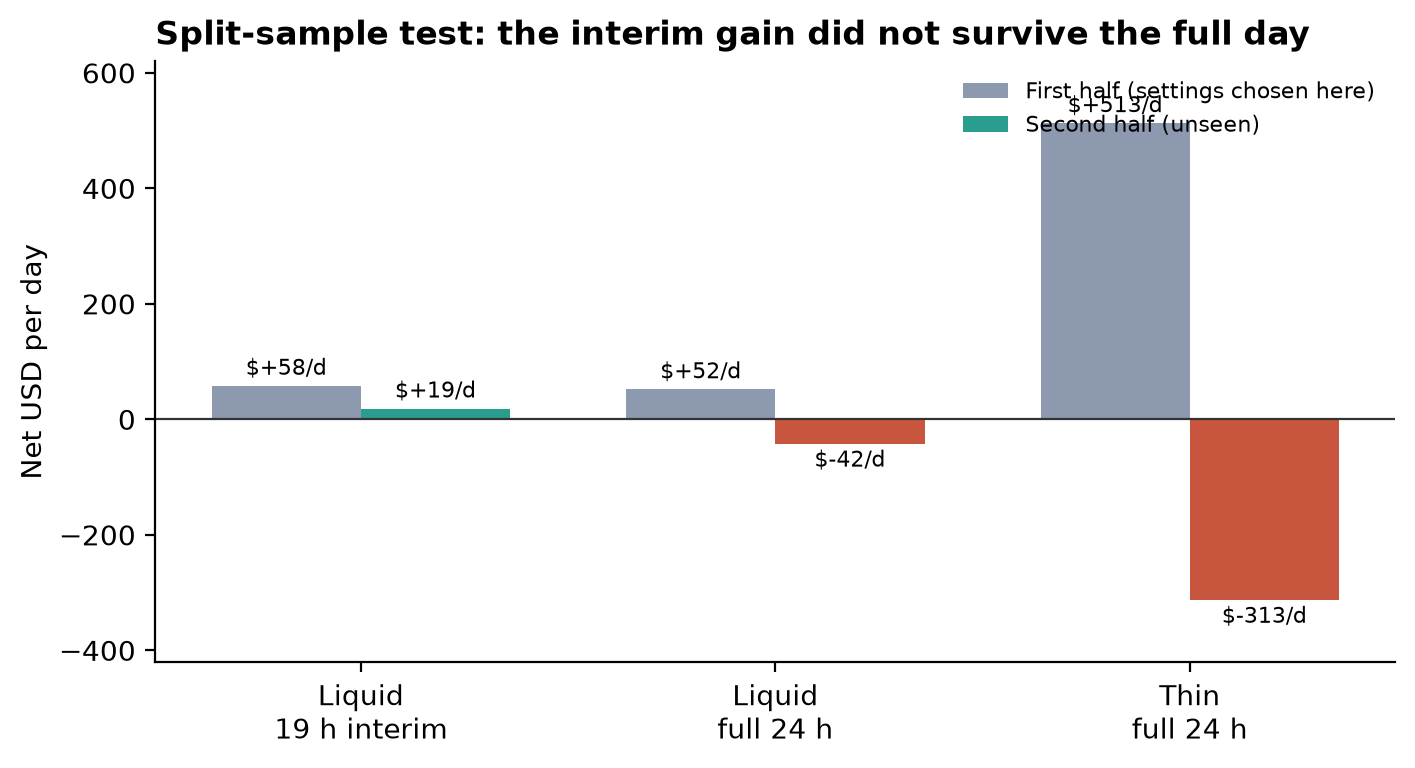
\includegraphics[width=0.8\linewidth]{walkforward-final}
\caption{Settings chosen per market on the first half and scored on the unseen second half.}
\end{figure}
\begin{table}[H]\centering\small
\begin{tabular}{@{}lrrrr@{}}
\toprule
Test & First half & Second half & Capital & Rate \\
\midrule
Liquid, per-market settings (19 h interim) & +\$57.83 & +\$18.54 & \$12,982 & +0.14\% \\
Liquid, per-market settings (full day) & +\$51.83 & $-$\$42.44 & \$12,975 & $-$0.33\% \\
Liquid, size capped at minimum & +\$13.21 & $-$\$10.44 & \$3,183 & $-$0.33\% \\
Liquid, one group setting (3 back, 4$\times$) & +\$4.18 & $-$\$17.87 & \$13,095 & $-$0.14\% \\
Thin, per-market settings (full day) & +\$512.69 & $-$\$312.91 & \$11,308 & $-$2.77\% \\
\bottomrule
\end{tabular}
\caption{Net USD per day. 29 of 40 liquid markets were positive in the second half; three lost \$71.44 between them.}
\end{table}

\section{Capital simulation}
For each budget, markets that were positive in the first half are funded in rank order at minimum size, then scaled to 2$\times$ and 4$\times$ while budget remains. The allocation is scored on the unseen second half.

\begin{figure}[H]\centering
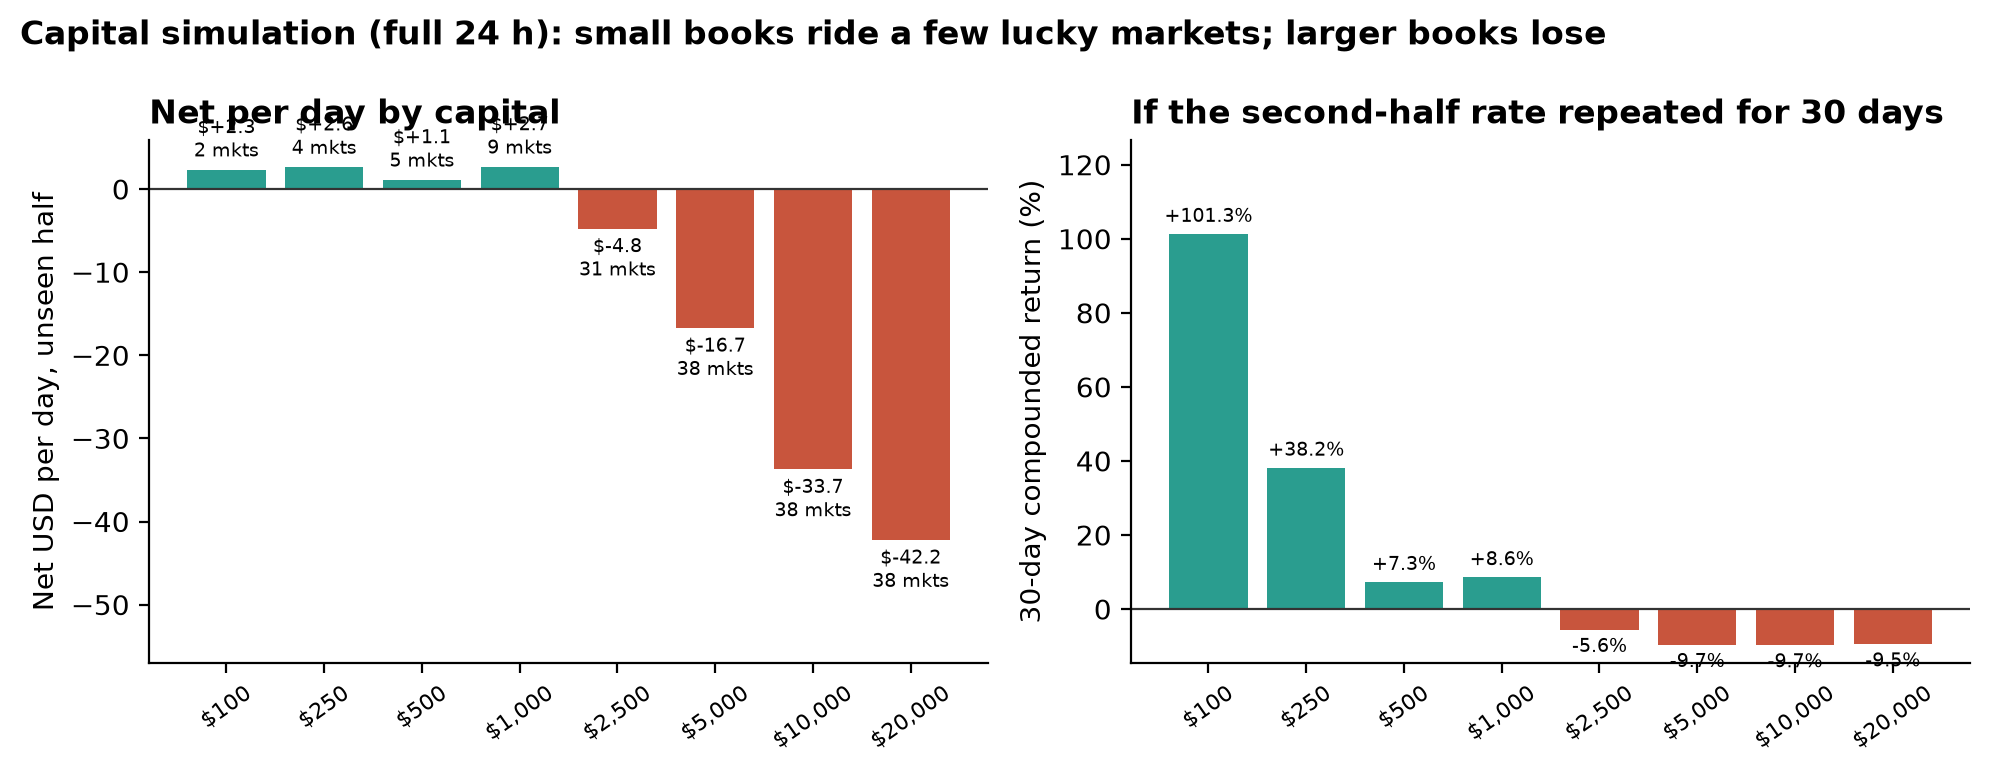
\includegraphics[width=\linewidth]{capital-sim-final}
\caption{Net per day and 30-day compounded return by capital, full 24-hour recording.}
\end{figure}
\begin{table}[H]\centering\small
\begin{tabular}{@{}rrrrrr@{}}
\toprule
Capital & Deployed & Markets & Net \$/day & Rate/day & 30 days, compounded \\
\midrule
\$100 & \$99 & 2 & +\$2.33 & +2.36\% & +101\% (+\$100) \\
\$250 & \$244 & 4 & +\$2.65 & +1.08\% & +38\% (+\$93) \\
\$500 & \$471 & 5 & +\$1.11 & +0.24\% & +7\% (+\$34) \\
\$1,000 & \$970 & 9 & +\$2.67 & +0.28\% & +9\% (+\$83) \\
\$2,500 & \$2,494 & 31 & $-$\$4.77 & $-$0.19\% & $-$6\% ($-$\$139) \\
\$5,000 & \$4,955 & 38 & $-$\$16.75 & $-$0.34\% & $-$10\% ($-$\$479) \\
\$10,000 & \$9,910 & 38 & $-$\$33.74 & $-$0.34\% & $-$10\% ($-$\$964) \\
\$20,000 & \$12,730 & 38 & $-$\$42.24 & $-$0.33\% & $-$9\% ($-$\$1,208) \\
\bottomrule
\end{tabular}
\caption{Small budgets fund only the 2--9 top-ranked markets, which happened to do well on the second half; this is a small sample and not evidence of a repeatable edge. Above \$2,500 the result converges on the portfolio rate of about $-$0.33\% per day. Compounded figures assume the rate repeats for 30 days.}
\end{table}

\section{Per-\$100 economics}
\begin{figure}[H]\centering
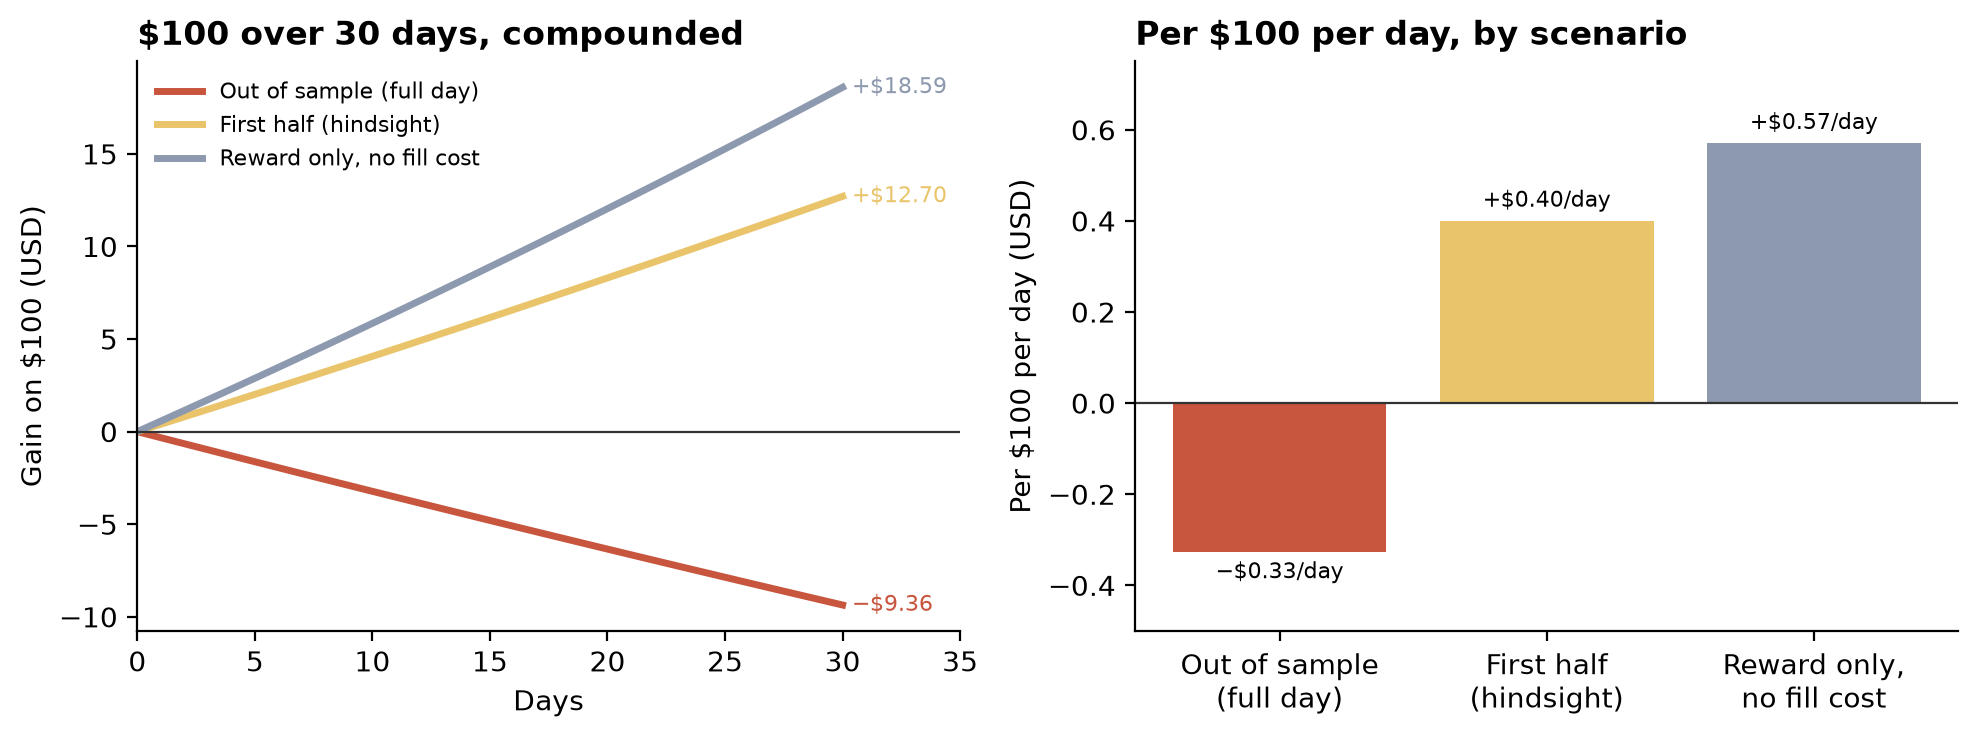
\includegraphics[width=\linewidth]{per100-final}
\caption{Per \$100 under three scenarios.}
\end{figure}
\begin{table}[H]\centering\small
\begin{tabularx}{\linewidth}{@{}p{3.8cm}rrY@{}}
\toprule
Scenario & Per \$100/day & 30 days & Basis \\
\midrule
Out of sample (full day) & $-$\$0.33 & $-$\$9.33 & Settings tested on unseen data; the figure to plan on \\
First half (hindsight) & +\$0.40 & +\$12.70 & Settings chosen and scored on the same data \\
Reward only, no fill cost & +\$0.57 & +\$18.60 & Best 10 liquid markets, snapshot, ignoring fills \\
\bottomrule
\end{tabularx}
\caption{Hindsight and reward-only figures are upper bounds, not forecasts.}
\end{table}

\section{Risks}
\begin{itemize}[leftmargin=1.2em]
  \item \textbf{Tail losses from adverse moves.} The decisive cost: a few news-driven moves outweighed a day of reward.
  \item \textbf{Overfitting.} Settings that looked best on one half lost on the other; the 19-hour interim overstated the result.
  \item \textbf{Thin and manipulable books.} Projected rewards there did not survive fills.
  \item \textbf{Concentration and capacity.} Rewards come from fixed pools (\$5,792 per day across the 40 liquid markets), so returns fall as size grows.
  \item \textbf{Model gaps.} Rewards are projected, queue position and routing are simplified, and benign fills are ignored.
  \item \textbf{Multi-outcome support and access.} Most of the best markets are multi-outcome, which the runner cannot quote; eligibility from the operating location is unverified.
\end{itemize}

\section{Gates before real capital}\label{sec:gates}
\begin{warn}
Current status: none of these gates has passed. Each is a condition for a capital decision.
\end{warn}
\begin{enumerate}[leftmargin=1.5em]
  \item Positive net out of sample across several days and splits, with tail losses included.
  \item Jump and news protection that pulls quotes before large moves, tested on recorded data.
  \item The same result from the full paper runner (queue, fills, inventory), not only the optimiser.
  \item Multi-outcome quoting implemented and tested; independent auditor updated.
  \item Live-path readiness, eligibility and wallet checks.
  \item Written sign-off on a canary size and stop rules.
\end{enumerate}

\section{Next steps}
\begin{enumerate}[leftmargin=1.5em]
  \item Add a jump filter to the optimiser (pull quotes when the midpoint moves more than a set amount, or volume spikes) and rerun the split test.
  \item Record further days and repeat the split test on each, including a test on a different day than the one used to choose settings.
  \item Add multi-outcome quoting to the paper runner and run it on the liquid markets.
\end{enumerate}

\section*{Reproducibility}
\small
\begin{itemize}[leftmargin=1.2em]
  \item Scan: \texttt{scripts/mm-reward-scan.mts}; recording: \texttt{scripts/mm-reward-projection.mts}, run \texttt{2026-10-20T18-40-36-481Z}.
  \item Optimiser: \texttt{scripts/mm\_param\_optimiser.py}; split test and capital simulation: \texttt{scripts/mm\_walkforward\_capital.py}, outputs in \texttt{final-20261021/}.
  \item Benchmark and fixes: \texttt{docs/MM\_POLYMAKER\_BENCHMARK\_2026-10-20.md}, \texttt{docs/MM\_RESET\_2026-10-20.md}, \texttt{docs/MM\_REWARD\_PROJECTION.md}.
\end{itemize}

\end{document}
